% TODO: rilettura
% TODO: Commento sugli intervalli di confidenza in relazione agli altri modelli
% TODO: Confronto con il percettrone
\chapter{Rete neurale} \label{chp:reteNeurale}
La precedente fase di analisi ha permesso di acquisire informazioni utili sulla
struttura del dataset e di conseguenza permettere la selezione di un modello
adatto a svolgere il compito di classificazione.

In questo capitolo verrà presentato uno dei tre modelli che sono stati realizzati
per svolgere il compito di classificazione, ovvero la rete neurale. Nello
specifico si andranno a presentare i passaggi che sono stati effettuati per la
realizzazione di questo modello, partendo dalla preparazione dei dati, passando
per la definizione della struttura della rete neurale, fino ad arrivare ai
risultati ottenuti.
\section{Preparazione dei dati}
Prima di passare alla presentazione della rete neurale nel dettaglio, risulta
necessario specificare come sono stati preparati i dati per l'addestramento della
rete neurale.

La prima operazione svolta sui dati è stata un operazione di standardizzazione,
ovvero per ogni feature è stata calcolata la media e la deviazione standard e
questi valori sono stati utilizzati per standardizzare i dati.

Eseguendo questa operazione i dati sono stati trasformati in modo tale che la
loro media sia 0 e la loro deviazione standard sia 1. Questa operazione è stata
eseguita per garantire che la rete neurale non sia influenzata da valori di input
con scale diverse.

La seconda operazione svolta sul dataset è stata la suddivisione in training set
e test set. Questa operazione è stata fatta per poter utilizzare una parte dei
dati per addestrare la rete neurale e una parte dei dati per valutare le
prestazioni della rete neurale. La suddivisione del dataset è stata effettuata
in modo tale che il training set contenesse il $80\%$ dei dati, mentre il test
set contenesse il $20\%$ dei dati.

Questa operazione è stata effettuata in modo da mantenere la stessa percentuale
di dati positivi e negativi in entrambi i set, con lo scopo di evitare che la
rete neurale sia addestrata su un dataset sbilanciato e di conseguenza non sia
in grado di generalizzare correttamente.
\section{Struttura della rete neurale}
Per definire la struttura della rete neurale sono stati utilizzati i risultati
ottenuti dalla fase di analisi a cui si è aggiunta una fase di grid search. Questa
fase è stata effettuata per valutare la combinazione migliore di iperparametri
per la rete neurale.

Dai risultati ottenuti dalla fase di analisi e dal dominio del problema, si è
scelto di utilizzare una rete con una struttura di dimensioni ridotte, in modo
tale da evitare l'overfitting.

Per svolgere il compito di classificazione si è scelto di utilizzare una rete
neurale feedforward, la cui struttura, a meno del layer di input e di output, è
stata definita attraverso un processo di grid search.

Dalla fase di analisi è stato selezionato un sottoinsieme di feature le quali
sono state utilizzate come input della rete neurale. Questo sottoinsieme è
composto da 5 elementi, il che ha permesso di definire la struttura del layer di
input della rete neurale. Questo primo strato è composto da 5 neuroni, in cui la
funzione di attivazione è stata definita come il resto delle funzioni di attivazione.
\subsection*{Ottimizzazione degli iperparametri}
Come già accennato in precedenza, la ricerca degli iperparametri della rete neurale
è stata effettuata attraverso un processo di grid search. Questo processo ha
permesso di valutare le prestazioni della rete neurale al variare della funzione
di attivazione, del numero di layer nascosti e del numero di neuroni per ogni
layer nascosto. Questo processo è stato effettuata attraverso una cross
validation a 5 fold, prendendo in considerazione solamente i dati del training set.

Visti i risultati ottenuti nella fase di analisi e la volontà di mantenere i
tempi di addestramento bassi, si è scelto di mantenere una struttura di dimensioni
ridotte per la rete neurale. Per questo motivo, l'operazione di grid search è
stata effettuata prendendo in considerazione un numero di neuroni per layer
tra 5, 10, 50, mentre il numero di layer nascosti è stato valutato tra 1 e 2.

Per quanto riguarda la funzione di attivazione, sono state valutate le seguenti
funzioni di attivazione:
\begin{itemize}
    \item \textit{ReLU}
    \item \textit{Leaky ReLU}
    \item \textit{sigmoid}
\end{itemize}

\begin{figure}[!ht]
    \centering
    \begin{subfigure}[b]{0.3\textwidth}
        \centering
        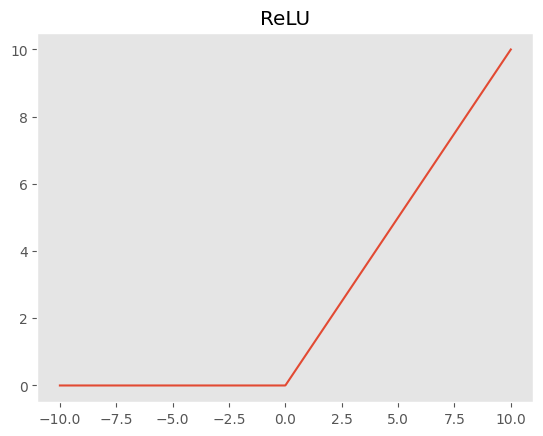
\includegraphics[width=\textwidth]{img/rete/relu.png}
        \caption{ReLU}
        \label{fig:relu}
    \end{subfigure}
    \hfill
    \begin{subfigure}[b]{0.3\textwidth}
        \centering
        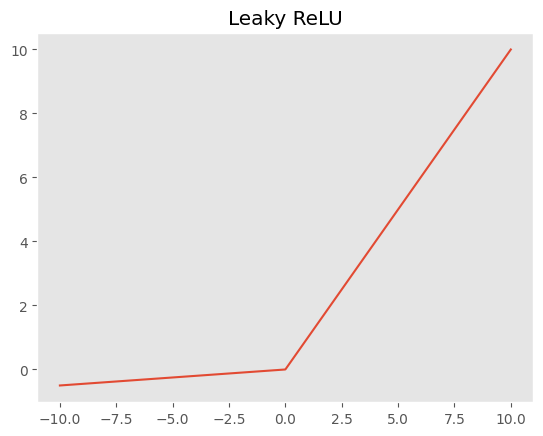
\includegraphics[width=\textwidth]{img/rete/leaky_relu.png}
        \caption{Leaky ReLU}
        \label{fig:leaky-relu}
    \end{subfigure}
    \hfill
    \begin{subfigure}[b]{0.3\textwidth}
        \centering
        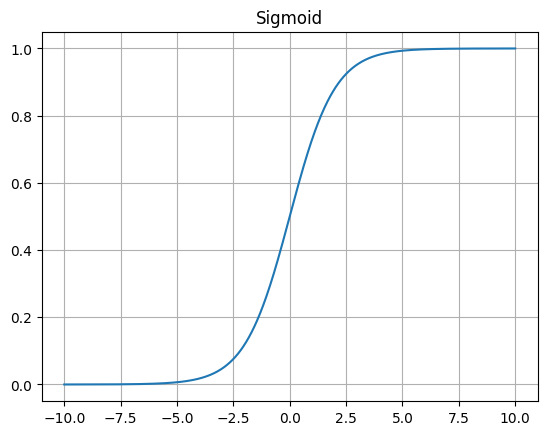
\includegraphics[width=\textwidth]{img/rete/sigmoid.png}
        \caption{Sigmoide}
        \label{fig:sigmoid}
    \end{subfigure}
    \caption{Funzioni di attivazione utilizzate nella fase di grid search}
    \label{fig:}
\end{figure}

Durante il processo di grid search, per ogni modello che è stato addestrato, sono
state raccolte delle informazioni relative all'accuratezza, al tempo di addestramento
richiesto. In aggiunta a queste informazioni, sono stati calcolati gli intervalli
di confidenza al $95\%$ per entrambe le misure.

Ottenuti i risultati, si è proceduto con l'analisi di questi, in modo tale da
definire la struttura della rete neurale. Per effettuare questa valutazione sono
state utilizzate le misure precedentemente citate.

Il modello selezionato è stato scelto in base al seguente criterio: si è scelto
il modello che ha ottenuto il valore più alto combinando, attraverso dei pesi,
i valori relativi all'accuratezza media, al tempo di addestramento medio e
agli intervalli di confidenza ottenuti. Per questa operazione si è scelto di
assegnare un peso maggiore all'accuratezza media ottenuta dalla cross validation
e al tempo di addestramento medio.

Nello specifico, sono stati utilizzati i seguenti pesi: 2 per l'accuratezza
media, 2 per il tempo di addestramento medio e 1 per gli intervalli di
confidenza. Questi pesi sono stati scelti in modo tale da dare più importanza
all'accuratezza media e al tempo di addestramento medio, in quanto sono le due
misure che permettono di valutare le prestazioni della rete neurale.

Per verificare la validità del modello scelto si è proceduto con il confronto tra
il modello che ha ottenuto la migliore accuratezza e il modello che ha ottenuto
il tempo di addestramento minore, ottenendo i risultati riportati in tabella \ref{tab:ris-grid-search}.
\begin{table}[ht]
    \centering
    \begin{tabular}{@{}lcc@{}}
        \toprule
        \rowcolor[HTML]{EFEFEF}
        \multicolumn{1}{c}{\cellcolor[HTML]{EFEFEF}\textbf{Modello}} & \textbf{Accuratezza} & \textbf{Tempo di addestramento} \\ \midrule
        Tempo di addestramento minore                                & 98.1\%               & 0.96s                           \\
        Accuratezza maggiore                                         & 99.5\%               & 24.54s                          \\
        Modello scelto                                               & 98.7\%               & 2.7s                            \\ \bottomrule
    \end{tabular}
    \caption{Risultati ottenuti dalla fase di grid search}
    \label{tab:ris-grid-search}
\end{table}

Dai valori riportati nella tabella \ref{tab:ris-grid-search} si può notare che il
notare che il modello che è stato selezionato fornisce un buon compromesso tra
accuratezza e tempo di addestramento. Nello specifico, perdendo lo $0.8\%$ di
accuratezza si è ottenuto un tempo di addestramento minore di $21.84s$ secondi.

\subsection*{Definizione della struttura della rete neurale}
I risultati ottenuti dalla fase di grid search hanno permesso di definire la
struttura della rete neurale. In particolare, la rete neurale è composta da 1
layer di input, 1 layer nascosto e 1 layer di output.

Il layer nascosto è composto da 50 neuroni, in cui la funzione di attivazione è
la funzione Leaky ReLU.

Per concludere la descrizione della struttura della rete neurale, è necessario
specificare come è composto l'ultimo layer, ovvero quello di output. Vista la
natura del problema di classificazione, il layer di output è composto da un solo
neurone, in cui la funzione di attivazione è la funzione sigmoide \ref{fig:sigmoid}.
Questa scelta è dovuta al fatto che tale funzione restituisce un valore compreso
tra 0 e 1, il che permette di interpretare l'output della rete neurale come la
probabilità che l'input appartenga alla classe positiva.
\begin{equation}
    \sigma(x) = \frac{1}{1 + e^{-x}}
\end{equation}

La struttura della rete neurale è riassunta nella figura \ref{fig:strutturaReteNeurale}.
\begin{figure}[!ht]
    \centering
    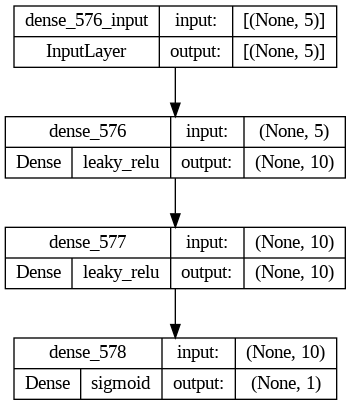
\includegraphics[width=0.3\textwidth]{img/rete/struttura_rete.png}
    \caption{Struttura della rete neurale}
    \label{fig:strutturaReteNeurale}
\end{figure}
\subsection*{Altri iperparametri} % TODO: titolo migliore
Oltre alla ricerca della struttura della rete neurale, la fase di grid search è
stata utilizzata per valutare l'algoritmo di ottimizzazione, il numero di epoche
e la dimensione del batch.

Per quanto riguarda l'algoritmo di ottimizzazione, il confronto è stato eseguito
tra \textit{Adam} e \textit{SGD}, mentre per il numero di epoche e la dimensione
del batch sono stati valutati i valori 100, 300 per il numero di epoche e 50,
100, 300 per la dimensione del batch.

I risultati ottenuti dalla fase di grid search hanno permesso di definire i valori
degli iperparametri che hanno permesso di ottenere i migliori risultati. In
particolare, l'algoritmo di ottimizzazione scelto è \textit{Adam}, mentre il
numero di epoche e la dimensione del batch sono stati impostati a 100 e 100
rispettivamente.

In questa fase è stato necessario definire la funzione di perdita. Si è scelta
la \textit{binary crossentropy} in quanto adatta a problemi di classificazione
binaria. La scelta di questa loss è dovuta alla natura del problema di
classificazione che si vuole risolvere.
\section{Addestramento della rete neurale}
La fase di addestramento della rete neurale è stata effettuata utilizzando il
training set precedentemente definito. L'addestramento della rete neurale è stato
effettuato utilizzando la libreria \textit{Keras} in quanto permette di definire
e addestrare reti neurali in modo intuitivo.
\section{Risultati}
Vista il dominio del problema, ovvero la classificazione di dati medici, si è
deciso di modificare manualmente il valore della soglia per la predizione
del tumore. Questa scelta è stata fatta in quanto si è voluto ridurre al minimo
il numero di falsi negativi, ovvero il numero di casi in cui il modello predice
l'assenza di tumore quando in realtà è presente.

Per realizzare questa operazione si è scelto di impostare il valore di threshold
a $0.3$, in modo tale da ridurre il numero di falsi negativi. Questa scelta è
stata fatta in quanto si è voluto dare più importanza al valore di richiamo, il
quale permette di valutare la capacità del modello di individuare i veri positivi.

Fatta questa precisazione, si può procedere con la presentazione dei risultati
ottenuti. Utilizzando i dati del test set, è stato possibile valutare le
prestazioni della rete neurale addestrata. In particolare, sono state calcolate
le seguenti metriche:
\begin{itemize}
    \item Accuratezza
    \item Precisione
    \item Richiamo
    \item F1 score
\end{itemize}
Oltre al calcolo di queste metriche, si è deciso di realizzare la curva ROC per
il modello e di rappresentare la matrice di confusione. Nella tabella
\ref{tab:risultatiReteNeurale} sono presentati i risultati ottenuti dal modello
addestrato.
\begin{table}[!ht]
    \centering
    \begin{tabular}{@{}cllll@{}}
        \toprule
        \rowcolor[HTML]{EFEFEF}
        \textbf{Metrica}                        & \textbf{Accuratezza}         & \textbf{Precisione}          & \textbf{Richiamo}            & \textbf{F1 score}            \\ \midrule
        \cellcolor[HTML]{EFEFEF}\textbf{Valore} & \multicolumn{1}{c}{98.80 \%} & \multicolumn{1}{c}{99.10 \%} & \multicolumn{1}{c}{98.21 \%} & \multicolumn{1}{c}{98.65 \%} \\ \bottomrule
    \end{tabular}
    \caption{Risultati ottenuti dal modello addestrato}
    \label{tab:risultatiReteNeurale}
\end{table}

Dai valori riportati nella tabella \ref{tab:risultatiReteNeurale} si può notare
che la rete neurale ha ottenuto dei valori delle metriche molto alti. Questo
comportamento è giustificato dal fatto che in fase di analisi è stato possibile
notare che le feature selezionate sono in grado di discriminare in modo efficace
le due classi.

In aggiunta al calcolo di queste metriche, è stata calcolata la matrice di confusione
per il modello addestrato. La matrice di confusione ottenuta è riportata in figura
\ref{fig:matriceConfusioneReteNeurale}.

\begin{figure}[!ht]
    \centering
    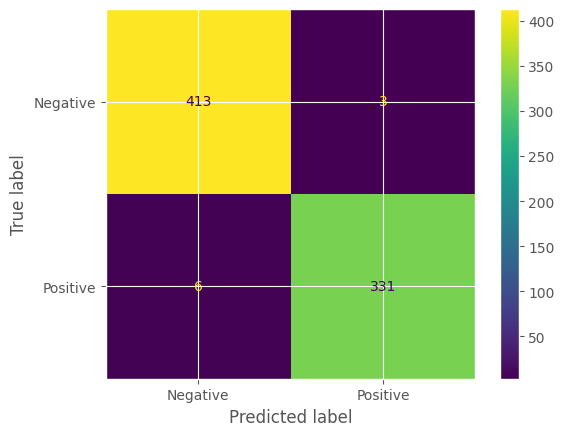
\includegraphics[width=0.5\textwidth]{img/rete/matrice_confusione.png}
    \caption{Matrice di confusione ottenuta dal modello addestrato}
    \label{fig:matriceConfusioneReteNeurale}
\end{figure}

Dalla matrice di confusione è possibile confermare i risultati ottenuti dalle
metriche calcolate in precedenza. Inoltre, avendo corretto manualmente il valore
della soglia, si è riusciti a ridurre il numero di falsi negativi, il che ha
permesso di aumentare il valore del richiamo.

Per concludere questa prima parte di analisi dei risultati, è stata realizzata
la curva ROC per il modello addestrato. La curva ROC ottenuta è riportata in
figura \ref{fig:curvaRocReteNeurale}. Oltre alla curva ROC è stata calcolata
l'area sotto la curva, la quale ha ottenuto un valore di $1.00$. Questo valore
ci permette di affermare che il modello addestrato si avvicina molto alla
perfetta classificazione.

\begin{figure}[!ht]
    \centering
    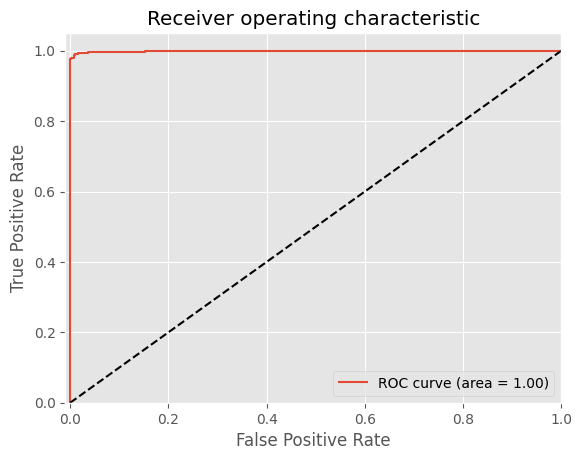
\includegraphics[width=0.5\textwidth]{img/rete/curva_roc.png}
    \caption{Curva ROC ottenuta dal modello addestrato}
    \label{fig:curvaRocReteNeurale}
\end{figure}
\subsection*{K-fold validation}
Per avere una visione più chiara dei risultati ottenuti, si è deciso di effettuare
una valutazione del modello attraverso 10 fold di cross validation. In questo
processo ogni modello che è stato addestrato è stato valutato attraverso le
metriche di accuratezza, precisione, richiamo e F1 score.

Per svolgere questa operazione è stato utilizzato il dataset completo, ovvero
senza alcuna suddivisione in training set e test set.

Anche per questa operazione è stato utilizzato il valore di threshold precedentemente
definito, ovvero $0.3$.

Sui risultati ottenuti da questo processo sono stati calcolati gli intervalli
di confidenza al $90\%$. I risultati ottenuti sono riportati in tabella
\ref{tab:risultatiCrossValidation}.

\begin{table}[ht]
    \centering
    \begin{tabular}{@{}lcc@{}}
        \toprule
        \rowcolor[HTML]{EFEFEF}
        \multicolumn{1}{c}{\cellcolor[HTML]{EFEFEF}\textbf{Metrica}} & \textbf{Valore Medio} & \textbf{Intervallo di confidenza} \\ \midrule
        Accuratezza                                                  & 98.19 \%              & [97.71\%, 98.67\%]                \\
        Precisione                                                   & 97.88 \%              & [97.16\%, 98.59\%]                \\
        Richiamo                                                     & 98.09 \%              & [97.19\%, 99.00\%]                \\
        F1 score                                                     & 97.97 \%              & [97.43\%, 98.52\%]                \\ \bottomrule
    \end{tabular}
    \caption{Risultati ottenuti dalla cross validation}
    \label{tab:risultatiCrossValidation}
\end{table}

Gli intervalli ottenuti sono stati successivamente rappresentati in un grafico
riportato in figura \ref{fig:risultatiCrossValidation}. Questo grafico permette
di avere una visione più chiara dei risultati ottenuti dalla cross validation.

\begin{figure}[!ht]
    \centering
    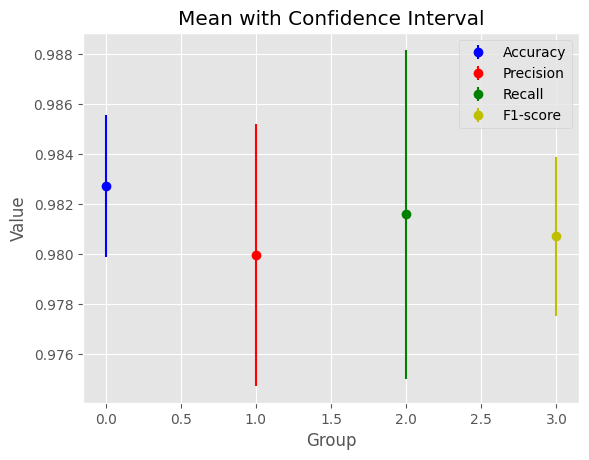
\includegraphics[width=0.5\textwidth]{img/rete/intervalli_confidenza.png}
    \caption{Risultati ottenuti dalla cross validation}
    \label{fig:risultatiCrossValidation}
\end{figure}
\section{Modello addestrato con PCA}
A puro scopo didattico, si è deciso di addestrare una rete neurale sul dataset
ottenuto attraverso la PCA. Per la precisione, si sono addestrati due modelli,
uno con gli stessi iperparametri del modello addestrato in precedenza e uno con
iperparametri che sono stati stimati attraverso un processo di grid search.

Il dataset ottenuto attraverso la PCA, descritto sella sezione \ref{sec:pca}, è
stato diviso in training set e test set in modo tale da mantenere la stessa
percentuale di dati positivi e negativi in entrambi i set.

Il meccanismo di grid search utilizzato per la ricerca degli iperparametri è
stato lo stesso utilizzato per il modello addestrato in precedenza. Anche
gli iperparametri valutati sono stati gli stessi.

I risultati ottenuti dai modelli addestrati sono riportati in tabella
\ref{tab:risultatiReteNeuralePCA}.

\begin{table}[ht]
    \centering
    \begin{tabular}{@{}lccccc@{}}
        \toprule
        \rowcolor[HTML]{EFEFEF}
        \multicolumn{1}{c}{\cellcolor[HTML]{EFEFEF}\textbf{Modello}} & \textbf{Accuratezza} & \textbf{F1} & \textbf{Precision} & \textbf{Recall} \\ \midrule
        Rete senza PCA                                               & 98.80\%              & 98.65\%     & 99.10\%            & 98.65\%         \\
        Rete con PCA                                                 &                      &             &                    &                 \\
        Rete con PCA e grid search                                   & 98.27\%              & 98.07\%     & 97.92\%            & 98.21\%         \\ \bottomrule
    \end{tabular}
    \caption{Risultati ottenuti dai modelli addestrati con PCA}
    \label{tab:risultatiReteNeuralePCA}
\end{table}

Per confrontare i modelli ottenuti con e senza PCA, sono state utilizzate, oltre
alle metriche precedentemente presentate, anche le curve ROC e gli intervalli di
confidenza. I risultati ottenuti sono riportati in figura \ref{fig:confrontoRisultatiPCA}.

\begin{figure}[!ht]
    \centering
    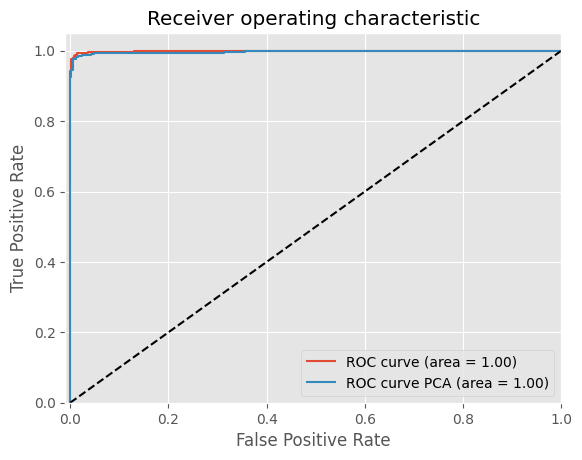
\includegraphics[width=0.5\textwidth]{img/rete/confrontoRoc.png}
    \caption{Confronto curve ROC tra il modello addestrato con e senza PCA}
    \label{fig:confrontoRisultatiPCA}
\end{figure}

Da questa figura si può notare che la differenza tra i due modelli è minima.
Entrambi i modelli si avvicinano molto alla perfetta classificazione. Si può
notare una differenza maggiore tra i due modelli osservando gli intervalli di
confidenza. In particolare, si può notare che il modello addestrato con PCA ha
un intervallo di confidenza più ampio rispetto al modello addestrato senza PCA.

Nella figura \ref{fig:intervalliConfidenzaPCA} sono riportati gli intervalli di
confidenza ottenuti dai modelli addestrati con e senza PCA. Da questa figura si
può notare che l'intervallo di confidenza ottenuto dal modello addestrato con
PCA, rappresentato dalla linea di colore rosso, è più ampio rispetto a quello 
ottenuto dal modello addestrato senza PCA, rappresentato dalla linea di colore blu.
\begin{figure}[!ht]
    \centering
    \begin{subfigure}[b]{0.4\textwidth}
        \centering
        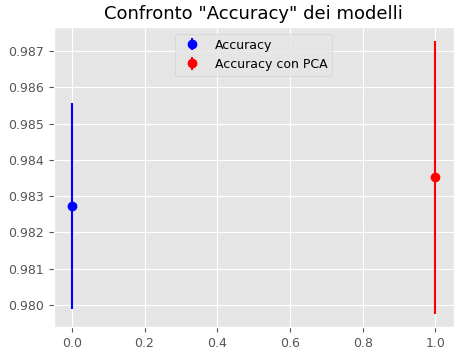
\includegraphics[width=\textwidth]{img/rete/intervalliAcc.png}
        \caption{Accuracy}
        \label{fig:acc}
    \end{subfigure}
    \hfill
    \begin{subfigure}[b]{0.4\textwidth}
        \centering
        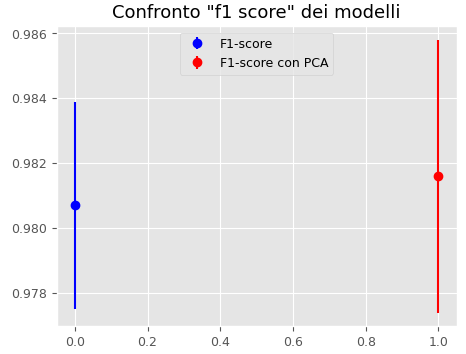
\includegraphics[width=\textwidth]{img/rete/intervalliF1.png}
        \caption{F1 score}
        \label{fig:f1}
    \end{subfigure}
    \hfill
    \begin{subfigure}[b]{0.4\textwidth}
        \centering
        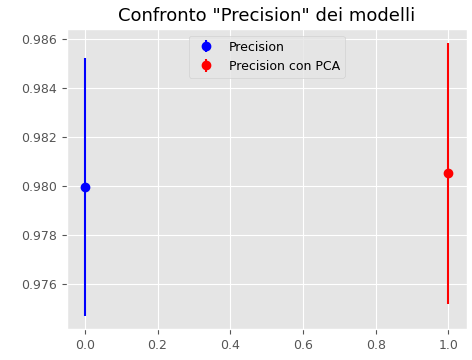
\includegraphics[width=\textwidth]{img/rete/intervalliPrecision.png}
        \caption{Precision}
        \label{fig:precision}
    \end{subfigure}
    \hfill
    \begin{subfigure}[b]{0.4\textwidth}
        \centering
        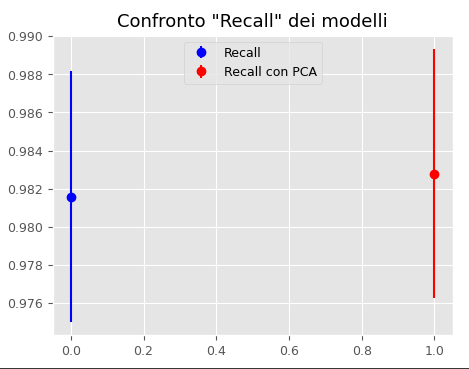
\includegraphics[width=\textwidth]{img/rete/intervalliRecall.png}
        \caption{Recall}
        \label{fig:recall}
    \end{subfigure}
    \caption{Intervalli di confidenza ottenuti dai modelli addestrati con e senza PCA}
    \label{fig:intervalliConfidenzaPCA}
\end{figure}
